% rtl_overview.tex -- RTL walkthrough of the systolic-array accelerator
% Build:  tectonic rtl_overview.tex      (or: pdflatex rtl_overview.tex, run twice)
\documentclass[aspectratio=169,11pt]{beamer}

\usepackage{tikz}
\usetikzlibrary{arrows.meta,positioning,shapes.geometric,fit,calc}
\usepackage{booktabs}
\usepackage{array}

% ---------------- look ----------------
\definecolor{pcb}{HTML}{0B2E33}      % dark board green
\definecolor{pcbmid}{HTML}{1F5C61}
\definecolor{tint}{HTML}{E6F0EF}
\definecolor{copper}{HTML}{B5651D}
\definecolor{ink}{HTML}{1F2A2E}
\definecolor{muted}{HTML}{5B6B70}

\usetheme{default}
\setbeamercolor{background canvas}{bg=white}
\setbeamercolor{frametitle}{fg=pcb}
\setbeamercolor{normal text}{fg=ink}
\setbeamercolor{structure}{fg=pcbmid}
\setbeamercolor{alerted text}{fg=copper}
\setbeamerfont{frametitle}{series=\bfseries,size=\Large}
\setbeamertemplate{navigation symbols}{}
\setbeamertemplate{itemize item}{\color{copper}$\blacktriangleright$}
\setbeamertemplate{itemize subitem}{\color{pcbmid}--}
\setbeamertemplate{footline}{\hfill\color{muted}\scriptsize\insertframenumber\hspace{1.2em}\vspace{0.6em}}

\newcommand{\file}[1]{\texttt{\textcolor{copper}{#1}}}
\newcommand{\sig}[1]{\texttt{#1}}

\tikzset{
  mod/.style   ={draw=pcbmid, fill=tint, rounded corners=3pt, thick, align=center,
                 font=\footnotesize, inner sep=4pt},
  hot/.style   ={draw=copper, fill=copper!12, rounded corners=3pt, thick, align=center,
                 font=\footnotesize, inner sep=4pt},
  ext/.style   ={draw=muted, dashed, rounded corners=3pt, align=center, font=\footnotesize},
  wire/.style  ={-{Stealth[length=2mm]}, thick, copper},
  wireb/.style ={-{Stealth[length=2mm]}, thick, pcbmid},
  lbl/.style   ={font=\scriptsize\ttfamily, fill=white, inner sep=1pt},
  st/.style    ={circle, draw=pcbmid, fill=tint, thick, minimum size=11mm,
                 font=\scriptsize\bfseries, align=center},
}

% file-tree helpers (slide 4)
\newcommand{\hn}[4]{\node[anchor=west,inner sep=0.5pt,font=\scriptsize\ttfamily,text=#4] at (#1*6,-#2*3.9) {#3};}
\newcommand{\role}[2]{\node[anchor=west,inner sep=0pt,font=\tiny,text=muted] at (40,-#1*3.9) {#2};}
\newcommand{\stub}[2]{\draw[pcbmid,thick] (#1*6-4,-#2*3.9) -- (#1*6-0.6,-#2*3.9);}
\newcommand{\trunk}[3]{\draw[pcbmid,thick] (#1*6+2,-#2*3.9-1.8) -- (#1*6+2,-#3*3.9);}

\title{\textcolor{pcb}{RTL of the Systolic-Array Accelerator}}
\subtitle{How the hardware works: components, values, and how data moves from file to file}
\author{Group project \textperiodcentered{} DE10-Lite (Intel MAX~10)}
\date{}

\begin{document}

% =====================================================================
\begin{frame}
  \titlepage
  \centering\color{muted}\small
  Covers only the RTL in \file{rtl/}. Values shown for the default build:
  \textbf{N = 4}, K\_MAX = 64 (target N = 8).
\end{frame}

% =====================================================================
\begin{frame}{How to learn RTL (the method behind these slides)}
  \begin{columns}[T]
    \column{0.55\textwidth}
    \begin{enumerate}
      \item \textbf{Think in hardware, not code.} Every \sig{always\_ff} is a set of
            flip-flops; every \sig{assign} is wires and gates. Draw it first.
      \item \textbf{Big picture first:} which blocks exist and what connects them.
      \item \textbf{Follow one piece of data} end to end (this deck: one matrix job).
      \item \textbf{Then zoom into one module} at a time, bottom to top.
      \item \textbf{Run its test, open the waveform,} match each signal to the drawing.
      \item \textbf{Break one line on purpose} and see which test catches it.
    \end{enumerate}
    \column{0.42\textwidth}
    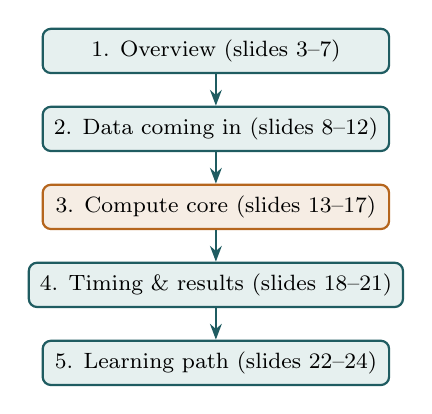
\begin{tikzpicture}[node distance=4mm]
      \node[mod, minimum width=44mm] (a) {1. Overview (slides 3--7)};
      \node[mod, minimum width=44mm, below=of a] (b) {2. Data coming in (slides 8--12)};
      \node[hot, minimum width=44mm, below=of b] (c) {3. Compute core (slides 13--17)};
      \node[mod, minimum width=44mm, below=of c] (d) {4. Timing \& results (slides 18--21)};
      \node[mod, minimum width=44mm, below=of d] (e) {5. Learning path (slides 22--24)};
      \foreach \x/\y in {a/b,b/c,c/d,d/e} \draw[wireb] (\x) -- (\y);
    \end{tikzpicture}
  \end{columns}
\end{frame}

% =====================================================================
\begin{frame}{The big picture: what happens in one job}
  \centering
  \resizebox{0.97\textwidth}{!}{%
  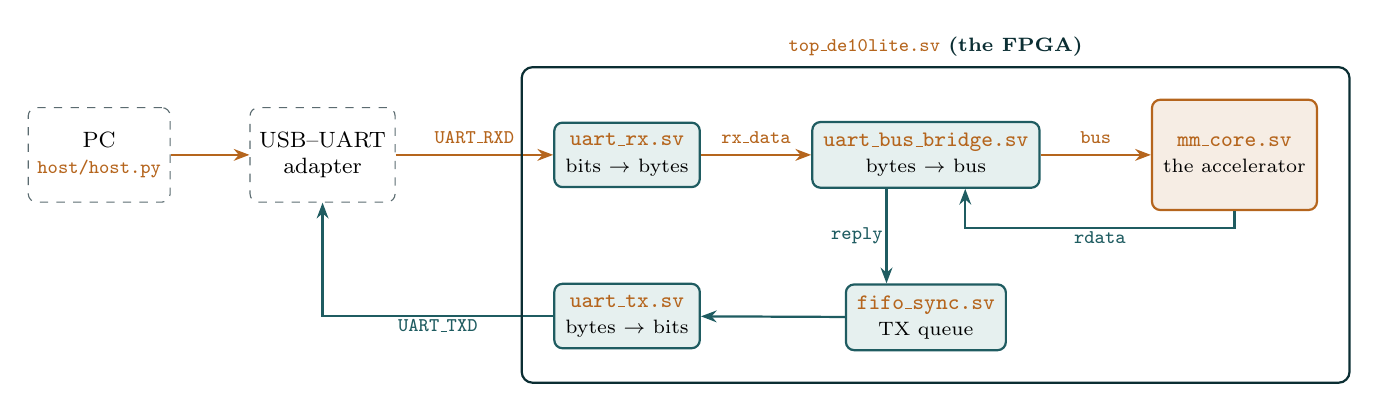
\begin{tikzpicture}[node distance=8mm and 14mm]
    \node[ext, minimum height=12mm] (pc) {PC\\\scriptsize\file{host/host.py}};
    \node[ext, right=10mm of pc, minimum height=12mm] (usb) {USB--UART\\adapter};
    \node[mod, right=20mm of usb] (rx) {\file{uart\_rx.sv}\\\scriptsize bits $\to$ bytes};
    \node[mod, right=of rx] (br) {\file{uart\_bus\_bridge.sv}\\\scriptsize bytes $\to$ bus};
    \node[hot, right=of br, minimum height=14mm] (core) {\file{mm\_core.sv}\\\scriptsize the accelerator};
    \node[mod, below=12mm of rx] (tx) {\file{uart\_tx.sv}\\\scriptsize bytes $\to$ bits};
    \node[mod, below=12mm of br] (fifo) {\file{fifo\_sync.sv}\\\scriptsize TX queue};
    \draw[wire] (pc) -- (usb);
    \draw[wire] (usb) -- node[lbl,above=1mm]{UART\_RXD} (rx);
    \draw[wire] (rx) -- node[lbl,above=1mm]{rx\_data} (br);
    \draw[wire] (br) -- node[lbl,above=1mm]{bus} (core);
    \draw[wireb] (core.south) |- node[lbl,below,pos=0.75]{rdata} ([xshift=5mm,yshift=-5mm]br.south) -- ([xshift=5mm]br.south);
    \draw[wireb] ([xshift=-5mm]br.south) -- node[lbl,left]{reply} ([xshift=-5mm]fifo.north);
    \draw[wireb] (fifo) -- (tx);
    \draw[wireb] (tx.west) -| node[lbl,below,pos=0.25]{UART\_TXD} (usb.south);
    \node[draw=pcb, thick, rounded corners, inner sep=4mm,
          fit=(rx)(br)(core)(tx)(fifo), label={[font=\scriptsize\bfseries,text=pcb]above:\file{top\_de10lite.sv} (the FPGA)}] {};
  \end{tikzpicture}}
  \vspace{2mm}
  \begin{enumerate}\small
    \item PC sends matrices \textbf{A} and \textbf{B} as UART bytes $\to$ the bridge turns them into
          \textbf{register-bus writes}.
    \item PC writes \sig{CTRL.START} $\to$ the core multiplies: $C = A \times B$.
    \item PC reads \textbf{C} and the \textbf{performance counters} back the same way.
  \end{enumerate}
\end{frame}

% =====================================================================
\begin{frame}{Module hierarchy: which file instantiates which}
  \begin{columns}[T]
    \column{0.62\textwidth}
    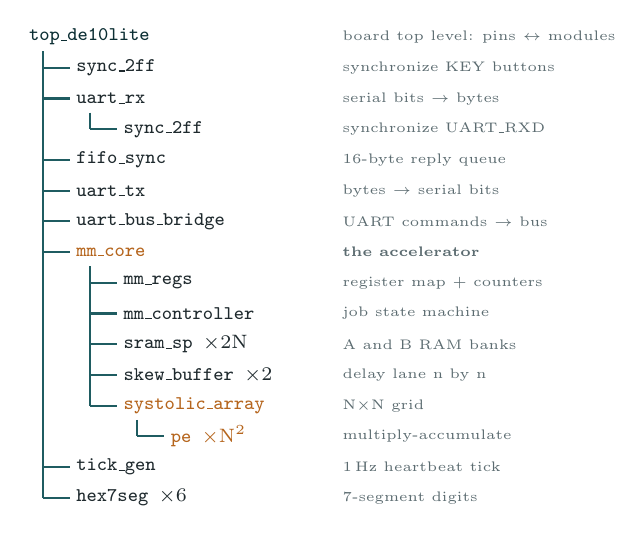
\begin{tikzpicture}[x=1mm,y=1mm]
      \trunk{0}{0}{15} \trunk{1}{2}{3} \trunk{1}{7}{12} \trunk{2}{12}{13}
      \hn{0}{0}{\textbf{top\_de10lite}}{pcb}                        \role{0}{board top level: pins $\leftrightarrow$ modules}
      \stub{1}{1}  \hn{1}{1}{sync\_2ff}{ink}                          \role{1}{synchronize KEY buttons}
      \stub{1}{2}  \hn{1}{2}{uart\_rx}{ink}                           \role{2}{serial bits $\to$ bytes}
      \stub{2}{3}  \hn{2}{3}{sync\_2ff}{ink}                          \role{3}{synchronize UART\_RXD}
      \stub{1}{4}  \hn{1}{4}{fifo\_sync}{ink}                         \role{4}{16-byte reply queue}
      \stub{1}{5}  \hn{1}{5}{uart\_tx}{ink}                           \role{5}{bytes $\to$ serial bits}
      \stub{1}{6}  \hn{1}{6}{uart\_bus\_bridge}{ink}                  \role{6}{UART commands $\to$ bus}
      \stub{1}{7}  \hn{1}{7}{\textbf{mm\_core}}{copper}               \role{7}{\textbf{the accelerator}}
      \stub{2}{8}  \hn{2}{8}{mm\_regs}{ink}                           \role{8}{register map + counters}
      \stub{2}{9}  \hn{2}{9}{mm\_controller}{ink}                     \role{9}{job state machine}
      \stub{2}{10} \hn{2}{10}{sram\_sp \textrm{$\times$2N}}{ink}      \role{10}{A and B RAM banks}
      \stub{2}{11} \hn{2}{11}{skew\_buffer \textrm{$\times$2}}{ink}   \role{11}{delay lane n by n}
      \stub{2}{12} \hn{2}{12}{systolic\_array}{copper}                \role{12}{N$\times$N grid}
      \stub{3}{13} \hn{3}{13}{pe \textrm{$\times$N$^2$}}{copper}      \role{13}{multiply-accumulate}
      \stub{1}{14} \hn{1}{14}{tick\_gen}{ink}                         \role{14}{1\,Hz heartbeat tick}
      \stub{1}{15} \hn{1}{15}{hex7seg \textrm{$\times$6}}{ink}        \role{15}{7-segment digits}
    \end{tikzpicture}
    \column{0.36\textwidth}
    \small
    \textbf{Where the files are}
    \begin{itemize}
      \item \file{rtl/top/}: board level\\ \scriptsize top\_de10lite, uart\_bus\_bridge
      \item \file{rtl/core/}: the accelerator\\ \scriptsize mm\_core, mm\_regs, mm\_controller,
            sram\_sp, skew\_buffer, systolic\_array, pe
      \item \file{rtl/common/}: helpers\\ \scriptsize uart\_rx/tx, fifo\_sync, sync\_2ff,
            tick\_gen, hex7seg
    \end{itemize}
    \vspace{2mm}
    For N = 4: \textbf{16} PEs, \textbf{8} RAMs, \textbf{2} skew buffers.\\
    For N = 8: \textbf{64} PEs, \textbf{16} RAMs.
  \end{columns}
\end{frame}

% =====================================================================
\begin{frame}{Parameters: the values that size everything}
  \centering\small
  \begin{tabular}{@{}l l l p{62mm}@{}}
    \toprule
    \textbf{Parameter} & \textbf{Value} & \textbf{Set in} & \textbf{What it controls} \\
    \midrule
    \sig{N}            & 4 (target 8)   & top\_de10lite  & array is N$\times$N; C is N$\times$N \\
    \sig{K\_MAX}       & 64             & top\_de10lite  & longest dot product; RAM depth \\
    \sig{DW}           & 8              & systolic\_array & operand width: signed int8 ($-128\ldots127$) \\
    \sig{AW}           & 32             & systolic\_array & accumulator width: signed int32 \\
    \sig{CLK\_HZ}      & 50\,000\,000   & top\_de10lite  & board clock (20\,ns period) \\
    \sig{BAUD}         & 115\,200       & top\_de10lite  & UART speed $\to$ \textbf{434} clocks per bit \\
    \sig{TIMEOUT\_CLKS}& 5\,000\,000    & uart\_bus\_bridge & 100\,ms: abandon a half-sent command \\
    \sig{DEPTH} (TX FIFO) & 16          & fifo\_sync     & response bytes waiting for the UART \\
    \sig{VERSION}      & 0x0001         & mm\_core       & read back through the INFO register \\
    \bottomrule
  \end{tabular}
  \vspace{3mm}

  \raggedright\footnotesize
  Parameters flow \textbf{down} the hierarchy: \sig{top\_de10lite \#(.N(4))} $\to$
  \sig{mm\_core \#(.N(N))} $\to$ \sig{systolic\_array \#(.N(N))}. Change N once at the top and every
  width below follows.
\end{frame}

% =====================================================================
\begin{frame}{Derived widths: \sig{\$clog2} turns parameters into bit counts}
  \centering\small
  \begin{tabular}{@{}l l c c l@{}}
    \toprule
    \textbf{Name} & \textbf{Formula} & \textbf{N=4} & \textbf{N=8} & \textbf{Used for} \\
    \midrule
    \sig{KW}  & \$clog2(K\_MAX)        & 6  & 6  & RAM address (k = 0..63) \\
    \sig{KL}  & \$clog2(K\_MAX+1)      & 7  & 7  & k\_len (1..64 needs 7 bits) \\
    \sig{LW}  & \$clog2(N)             & 2  & 3  & which lane (row/column) \\
    \sig{c\_idx} & \$clog2(N$\cdot$N)  & 4  & 6  & which C element to read \\
    \sig{TW}  & \$clog2(K\_MAX+2N)     & 7  & 7  & controller step counter t \\
    \midrule
    \sig{a\_in}, \sig{b\_in} & N$\cdot$8        & 32  & 64   & one column of A / row of B \\
    \sig{c\_out} & N$\cdot$N$\cdot$32           & 512 & 2048 & all accumulators, flattened \\
    \bottomrule
  \end{tabular}
  \vspace{3mm}

  \raggedright\footnotesize
  \textbf{Flat vectors:} lane n of a bus is \sig{[n*W +: W]}. Example: \sig{a\_in[2*8 +: 8]} = bits
  23:16 = row 2. Element C(i,j) is \sig{c\_out[(i*N+j)*32 +: 32]}.
\end{frame}

% =====================================================================
\begin{frame}{Signals that cross file boundaries (N = 4)}
  \centering\scriptsize
  \resizebox{\textwidth}{!}{%
  \begin{tabular}{@{}l l l l@{}}
    \toprule
    \textbf{From} & \textbf{To} & \textbf{Signals [width]} & \textbf{Meaning} \\
    \midrule
    pin UART\_RXD & uart\_rx & rx [1] & serial bits from the PC \\
    uart\_rx & uart\_bus\_bridge & rx\_data [8], rx\_valid & one received byte \\
    uart\_bus\_bridge & mm\_regs & bus\_valid, bus\_write, bus\_addr [16], bus\_wdata [32] & bus request \\
    mm\_regs & uart\_bus\_bridge & bus\_ready, bus\_rvalid, bus\_rdata [32] & accept / read data \\
    uart\_bus\_bridge & fifo\_sync $\to$ uart\_tx & tx\_data [8], tx\_push / tx\_full & response bytes \\
    mm\_regs & mm\_controller & start, k\_len [7] & begin a job of length K \\
    mm\_regs & sram\_sp (8$\times$) & wr\_en, wr\_sel, wr\_lane [2], wr\_addr [6], wr\_data [8] & load A / B \\
    mm\_controller & sram\_sp & rd\_addr [6] (when busy) & read column k \\
    mm\_controller & skew, array & clear, array\_en & zero / run the array \\
    mm\_controller & mm\_regs & busy, done, all\_active, rd\_en & status + counter events \\
    sram\_sp & skew\_buffer & a\_col, b\_row [32] (zero when not valid) & A[.][k], B[k][.] \\
    skew\_buffer & systolic\_array & a\_skew, b\_skew [32] & diagonal wavefront \\
    systolic\_array & pe (16$\times$) & a\_in, b\_in [8] per PE & operands \\
    systolic\_array & mm\_core $\to$ mm\_regs & c\_out [512] $\to$ c\_data [32] via c\_idx [4] & result C \\
    mm\_core & top\_de10lite & busy, done, state [3], perf\_compute [32] & LEDs and HEX \\
    \bottomrule
  \end{tabular}}
\end{frame}

% =====================================================================
\begin{frame}{Step 1 --- a byte arrives: \file{uart\_rx.sv}}
  \begin{columns}[T]
    \column{0.52\textwidth}\small
    \begin{itemize}
      \item The pin is \textbf{asynchronous}: first through \file{sync\_2ff.sv} (2 flip-flops)
            to avoid metastability.
      \item Line idles at 1. A \textbf{falling edge} = start bit.
      \item Wait \textbf{217} clocks (half a bit) $\to$ middle of the start bit, check it is still 0.
      \item Sample every \textbf{434} clocks $\to$ middle of each of the 8 data bits (LSB first).
      \item Check the stop bit is 1 $\to$ pulse \sig{valid} for one cycle with \sig{data}.
            Else pulse \sig{frame\_err} (LEDR5).
    \end{itemize}
    \column{0.45\textwidth}
    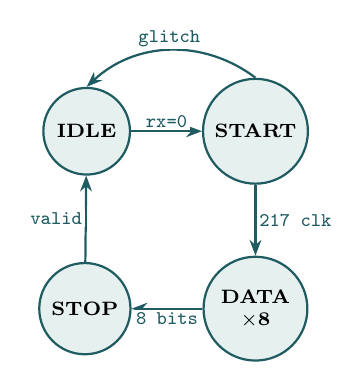
\begin{tikzpicture}[node distance=9mm]
      \node[st] (i) {IDLE};
      \node[st, right=of i] (s) {START};
      \node[st, below=of s] (d) {DATA\\$\times$8};
      \node[st, left=of d] (p) {STOP};
      \draw[wireb] (i) -- node[lbl,above]{rx=0} (s);
      \draw[wireb] (s) -- node[lbl,right]{217 clk} (d);
      \draw[wireb] (d) -- node[lbl,below]{8 bits} (p);
      \draw[wireb] (p) -- node[lbl,left]{valid} (i);
      \draw[wireb] (s.north) to[bend right=40] node[lbl,above]{glitch} (i.north);
    \end{tikzpicture}\\[2mm]
    \scriptsize\color{muted} 50\,000\,000 / 115\,200 = 434.03 $\to$ 434 clocks per bit.
    One byte = 10 bits $\approx$ 4\,340 clocks $\approx$ 87\,\textmu s.
  \end{columns}
\end{frame}

% =====================================================================
\begin{frame}{Step 2 --- bytes become bus transactions: \file{uart\_bus\_bridge.sv}}
  \begin{columns}[T]
    \column{0.46\textwidth}\scriptsize
    \begin{tabular}{@{}l l l@{}}
      \toprule
      \textbf{Cmd} & \textbf{Bytes in} & \textbf{Reply} \\
      \midrule
      \texttt{W} & addr(2) data(4) & \texttt{K} \\
      \texttt{R} & addr(2) & data(4) \\
      \texttt{B} & addr(2) len(2) + len bytes & \texttt{K} \\
      \texttt{D} & addr(2) len(2) & len bytes \\
      \texttt{P} & --- & \texttt{K} N K\_MAX \\
      other & --- & \texttt{E} (LEDR6) \\
      \bottomrule
    \end{tabular}\\[2mm]
    All fields little-endian. Block write \texttt{B} sends one bus write per byte at
    addr + n. If the PC stops mid-command for 100\,ms $\to$ abandon (LEDR7).
    \column{0.52\textwidth}
    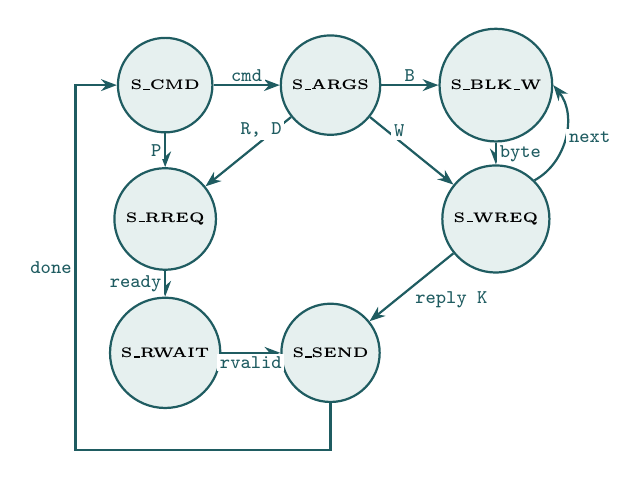
\begin{tikzpicture}[x=21mm,y=17mm]
      \tikzset{st2/.style={st, minimum size=12mm, font=\tiny\bfseries}}
      \node[st2] (c)  at (0,0)  {S\_CMD};
      \node[st2] (a)  at (1,0)  {S\_ARGS};
      \node[st2] (b)  at (2,0)  {S\_BLK\_W};
      \node[st2] (r)  at (0,-1) {S\_RREQ};
      \node[st2] (w)  at (2,-1) {S\_WREQ};
      \node[st2] (rw) at (0,-2) {S\_RWAIT};
      \node[st2] (s)  at (1,-2) {S\_SEND};
      \draw[wireb] (c) -- node[lbl,above]{cmd} (a);
      \draw[wireb] (a) -- node[lbl,above]{B} (b);
      \draw[wireb] (a) -- node[lbl,above,pos=0.35]{W} (w);
      \draw[wireb] (b) -- node[lbl,right]{byte} (w);
      \draw[wireb] (a) -- node[lbl,above,pos=0.35]{R, D} (r);
      \draw[wireb] (c) -- node[lbl,left]{P} (r);
      \draw[wireb] (r) -- node[lbl,left]{ready} (rw);
      \draw[wireb] (rw) -- node[lbl,below]{rvalid} (s);
      \draw[wireb] (w) -- node[lbl,below right]{reply K} (s);
      \draw[wireb] (w.north east) to[bend right=50] node[lbl,right]{next} (b.east);
      \draw[wireb] (s.south) -- ++(0,-0.35) -| node[lbl,left,pos=0.75]{done} ($(c.west)+(-0.25,0)$) -- (c.west);
    \end{tikzpicture}
  \end{columns}
\end{frame}

% =====================================================================
\begin{frame}{Step 3 --- the register bus (valid/ready handshake)}
  \begin{columns}[T]
    \column{0.5\textwidth}
    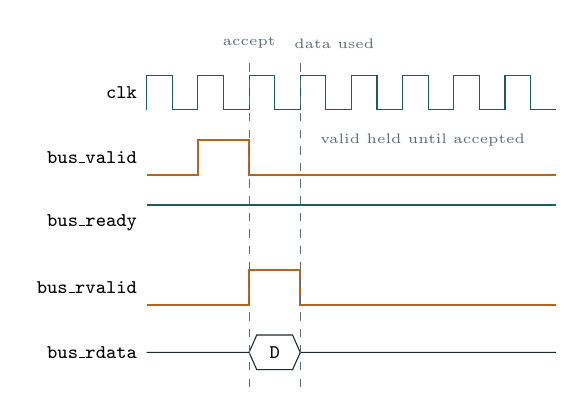
\begin{tikzpicture}[x=6.5mm,y=5.5mm, font=\scriptsize\ttfamily]
      % clock
      \node[left] at (0,6) {clk};
      \foreach \t in {0,...,7} \draw[pcbmid] (\t,5.6) -- (\t,6.4) -- (\t+0.5,6.4) -- (\t+0.5,5.6) -- (\t+1,5.6);
      \node[left] at (0,4.5) {bus\_valid};
      \draw[copper,thick] (0,4.1) -- (1,4.1) -- (1,4.9) -- (2,4.9) -- (2,4.1) -- (8,4.1);
      \node[left] at (0,3) {bus\_ready};
      \draw[pcbmid,thick] (0,3.4) -- (8,3.4);
      \node[left] at (0,1.5) {bus\_rvalid};
      \draw[copper,thick] (0,1.1) -- (2,1.1) -- (2,1.9) -- (3,1.9) -- (3,1.1) -- (8,1.1);
      \node[left] at (0,0) {bus\_rdata};
      \draw[ink] (0,0) -- (2,0) -- (2.15,0.4) -- (2.85,0.4) -- (3,0) -- (8,0);
      \draw[ink] (2,0) -- (2.15,-0.4) -- (2.85,-0.4) -- (3,0);
      \node at (2.5,0) {D};
      \draw[dashed,muted] (2,-0.8) -- (2,6.8) node[above,font=\tiny]{accept};
      \draw[dashed,muted] (3,-0.8) -- (3,6.8) node[above right,font=\tiny,xshift=-2mm]{data used};
      \node[font=\tiny\rmfamily,text=muted,anchor=west] at (3.2,4.9) {valid held until accepted};
    \end{tikzpicture}
    \column{0.48\textwidth}\small
    \begin{itemize}
      \item A request is \textbf{accepted} on the clock edge where
            \sig{bus\_valid \&\& bus\_ready}.
      \item \textbf{Write:} takes effect at that same edge.
      \item \textbf{Read:} \sig{bus\_rdata} arrives with \sig{bus\_rvalid}
            \textbf{exactly 1 cycle later}.
      \item \sig{bus\_ready} drops only for the one cycle of a soft reset.
      \item Same bus is used by: the UART bridge (board), cocotb tests, the SystemC model,
            and the UVM driver (Phase~6).
    \end{itemize}
  \end{columns}
\end{frame}

% =====================================================================
\begin{frame}{Step 4 --- address decode and register map: \file{mm\_regs.sv}}
  \begin{columns}[T]
    \column{0.53\textwidth}\scriptsize
    \resizebox{\linewidth}{!}{%
    \begin{tabular}{@{}l l l@{}}
      \toprule
      \textbf{Address} & \textbf{Name} & \textbf{Meaning} \\
      \midrule
      0x0000 & CTRL & bit0 START, bit1 SOFT\_RESET \\
      0x0004 & STATUS & bit0 BUSY, bit1 DONE \\
      0x0008 & CFG\_K & K, 1..64 \\
      0x000C & INFO & N, K\_MAX, VERSION \\
      0x0010--0x0020 & PERF\_* & 5 counters (slide 12) \\
      0x1000 + i$\cdot$64 + k & A\_BUF & A[i][k], one byte \\
      0x2000 + k$\cdot$N + j & B\_BUF & B[k][j], one byte \\
      0x3000 + 4(i$\cdot$N + j) & C\_BUF & C[i][j], int32 \\
      \bottomrule
    \end{tabular}}\\[3mm]
    \footnotesize\textbf{Try it:} 0x1083 $\to$ region 1, offset 131 $\to$ row 131 $\gg$ 6 = 2,
    k = 131 \& 63 = 3 $\to$ \textbf{A[2][3]}.
    \column{0.44\textwidth}\small
    \textbf{How an address is split}\\[1mm]
    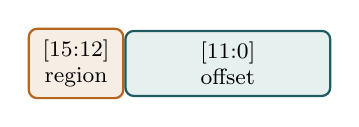
\begin{tikzpicture}
      \node[hot, minimum width=12mm] (r) {[15:12]\\region};
      \node[mod, right=0mm of r, minimum width=26mm] (o) {[11:0]\\offset};
    \end{tikzpicture}\\[2mm]
    \footnotesize
    \begin{itemize}
      \item region 0 = registers, \sig{reg\_sel = offset[7:2]}
      \item region 1 (A): lane = offset $\gg$ 6 = row i, addr = offset[5:0] = k
      \item region 2 (B): lane = offset[1:0] = col j, addr = offset $\gg$ 2 = k
      \item region 3 (C): \sig{c\_idx = offset[5:2]}
      \item A/B writes are \textbf{ignored while BUSY}.
    \end{itemize}
  \end{columns}
\end{frame}

% =====================================================================
\begin{frame}{Performance counters (inside \file{mm\_regs.sv})}
  \centering\small
  \resizebox{\textwidth}{!}{%
  \begin{tabular}{@{}l l l c c@{}}
    \toprule
    \textbf{Counter} & \textbf{Counts when} & \textbf{Formula} & \textbf{N=4, K=64} & \textbf{N=8, K=64} \\
    \midrule
    PERF\_TOTAL     & busy and not done       & K + 2N               & 72   & 80   \\
    PERF\_COMPUTE   & array\_en               & K + 2N $-$ 1         & 71   & 79   \\
    PERF\_FILLDRAIN & array\_en, not all\_active & compute $-$ max(0, K$-$2N+2) & 13 & 29 \\
    PERF\_MACS      & + N$^2$ per rd\_en      & N$^2\cdot$K          & 1\,024 & 4\,096 \\
    PERF\_IDLE      & not busy (saturates)    & depends on the host  & ---  & --- \\
    \bottomrule
  \end{tabular}}
  \vspace{4mm}

  \raggedright
  \begin{itemize}\small
    \item All counters (except IDLE) reset to 0 on \sig{START}, so each job is measured alone.
    \item \textbf{Utilisation} = MACS / (N$^2$ $\times$ COMPUTE) $\to$ 90.1\,\% (N=4), 81.0\,\% (N=8).
    \item HEX5..HEX0 on the board show \sig{PERF\_COMPUTE} of the last job.
    \item These same counters exist in the SystemC model $\to$ that is how HW and SW are compared.
  \end{itemize}
\end{frame}

% =====================================================================
\begin{frame}{Step 5 --- banked operand RAM: \file{sram\_sp.sv}}
  \begin{columns}[T]
    \column{0.5\textwidth}
    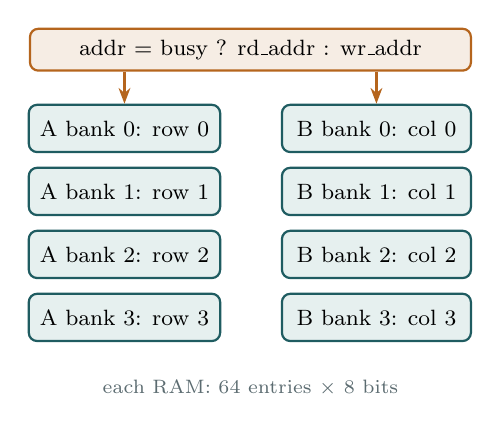
\begin{tikzpicture}[node distance=1.5mm]
      \foreach \i in {0,...,3} {
        \node[mod, minimum width=24mm, minimum height=6mm] (a\i) at (0,-\i*0.8) {A bank \i: row \i};
        \node[mod, minimum width=24mm, minimum height=6mm] (b\i) at (3.2,-\i*0.8) {B bank \i: col \i};
      }
      \node[hot, minimum width=56mm] (addr) at (1.6,1.0) {addr = busy ? rd\_addr : wr\_addr};
      \draw[wire] (addr.south -| a0.north) -- (a0.north);
      \draw[wire] (addr.south -| b0.north) -- (b0.north);
      \node[font=\scriptsize, text=muted] at (1.6,-3.3) {each RAM: 64 entries $\times$ 8 bits};
    \end{tikzpicture}
    \column{0.48\textwidth}\small
    \begin{itemize}
      \item The array needs \textbf{a whole column of A and a whole row of B every cycle}.
      \item So each row of A and each column of B gets its \textbf{own RAM} (N + N = 8 banks),
            all read at the \textbf{same address k}.
      \item \sig{sram\_sp} is written in the pattern Quartus maps to \textbf{M9K block RAM}.
      \item \textbf{1-cycle read latency:} data appears the cycle after \sig{rd\_en}, so
            \sig{rd\_valid} is \sig{rd\_en} delayed by one flip-flop.
      \item When \sig{rd\_valid = 0}, \textbf{zeros} are fed, so the accumulators do not change
            while the array fills and drains.
    \end{itemize}
  \end{columns}
\end{frame}

% =====================================================================
\begin{frame}{Step 6 --- the controller FSM: \file{mm\_controller.sv}}
  \begin{columns}[T]
    \column{0.55\textwidth}
    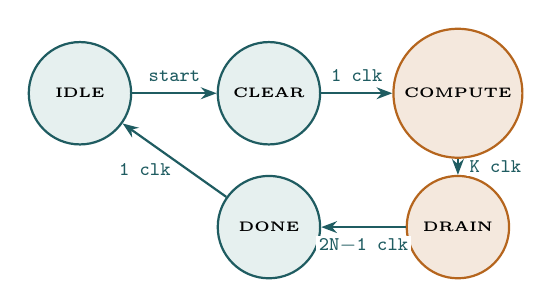
\begin{tikzpicture}[x=24mm,y=17mm]
      \tikzset{st3/.style={st, minimum size=13mm, font=\tiny\bfseries}}
      \node[st3] (i)  at (0,0)  {IDLE};
      \node[st3] (c)  at (1,0)  {CLEAR};
      \node[st3, fill=copper!15, draw=copper] (k)  at (2,0)  {COMPUTE};
      \node[st3, fill=copper!15, draw=copper] (d)  at (2,-1) {DRAIN};
      \node[st3] (dn) at (1,-1) {DONE};
      \draw[wireb] (i) -- node[lbl,above=1mm]{start} (c);
      \draw[wireb] (c) -- node[lbl,above=1mm]{1 clk} (k);
      \draw[wireb] (k) -- node[lbl,right=1mm]{K clk} (d);
      \draw[wireb] (d) -- node[lbl,below=1mm]{2N$-$1 clk} (dn);
      \draw[wireb] (dn) -- node[lbl,below left]{1 clk} (i);
    \end{tikzpicture}\\[2mm]
    \scriptsize
    \begin{tabular}{@{}l l@{}}
      \sig{busy} & state $\neq$ IDLE \\
      \sig{clear} & CLEAR: zero the array + skew \\
      \sig{rd\_en}, \sig{rd\_addr = t} & COMPUTE: read column t \\
      \sig{array\_en} & COMPUTE or DRAIN \\
      \sig{done} & DONE (1-cycle pulse) \\
      \sig{all\_active} & $2N-1 \le t \le K$ \\
    \end{tabular}
    \column{0.43\textwidth}\small
    \begin{itemize}
      \item One step counter \sig{t} runs 0 \ldots{} K + 2N $-$ 2 across COMPUTE and DRAIN.
      \item \textbf{COMPUTE} (t $<$ K): read address t from all 8 RAMs.
      \item \textbf{DRAIN}: no reads; zeros flow in while the last values travel to
            the bottom-right PE.
      \item Last product reaches PE(N$-$1,N$-$1) at t = K $-$ 1 + 1 (RAM) + 2(N$-$1) =
            \textbf{K + 2N $-$ 2}, the last DRAIN step. So C is complete when DONE is entered.
      \item LEDR[2:0] show the state number (0..4).
    \end{itemize}
  \end{columns}
\end{frame}

% =====================================================================
\begin{frame}{Step 7 --- skewing the inputs: \file{skew\_buffer.sv}}
  \begin{columns}[T]
    \column{0.5\textwidth}
    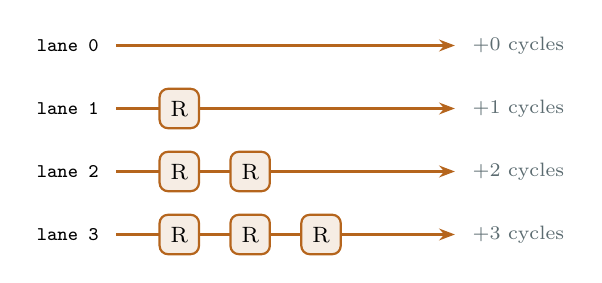
\begin{tikzpicture}[x=10mm,y=8mm]
      \foreach \n in {0,...,3} {
        \node[font=\scriptsize\ttfamily, anchor=east] at (0,-\n) {lane \n};
        \draw[wire] (0.1,-\n) -- (4.4,-\n);
        \ifnum\n>0
          \foreach \r in {1,...,\n} {
            \node[hot, minimum size=5mm, inner sep=0pt] at (\r*0.9,-\n) {R};
          }
        \fi
        \node[font=\scriptsize, anchor=west, text=muted] at (4.5,-\n) {+\n\ cycles};
      }
    \end{tikzpicture}
    \column{0.48\textwidth}\small
    \begin{itemize}
      \item The RAMs give A[0..3][k] all \textbf{in the same cycle}.
      \item But PE(i,j) must get A[i][k] and B[k][j] \textbf{at the same moment}, and A takes j hops,
            B takes i hops to get there.
      \item Fix: delay \textbf{lane n by n cycles} (a triangle of registers). Now everything meets
            on a diagonal ``wavefront''.
      \item N$\cdot$(N$-$1)/2 = \textbf{6} registers per buffer for N = 4 (28 for N = 8).
      \item Two copies: one for A (rows), one for B (columns).
    \end{itemize}
  \end{columns}
\end{frame}

% =====================================================================
\begin{frame}{Step 8 --- the grid: \file{systolic\_array.sv}}
  \begin{columns}[T]
    \column{0.5\textwidth}
    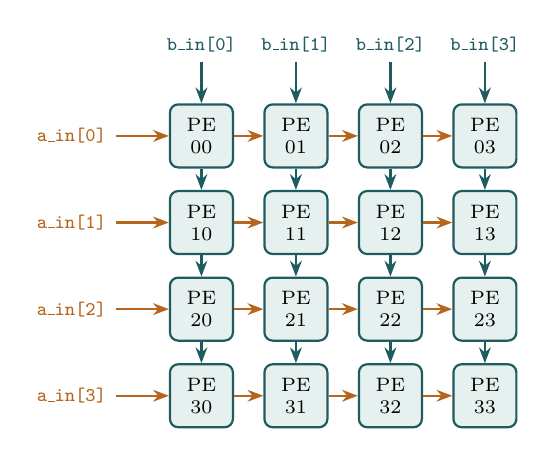
\begin{tikzpicture}[x=12mm,y=11mm]
      \foreach \i in {0,...,3} \foreach \j in {0,...,3} {
        \node[mod, minimum size=8mm, inner sep=1pt, font=\scriptsize] (p\i\j) at (\j,-\i) {PE\\\i\j};
      }
      \foreach \i in {0,...,3} {
        \draw[wire] (-0.9,-\i) node[left,font=\scriptsize\ttfamily]{a\_in[\i]} -- (p\i0);
        \draw[wireb] (\i,0.85) node[above,font=\scriptsize\ttfamily]{b\_in[\i]} -- (p0\i);
      }
      \foreach \i in {0,...,3} \foreach \j/\jn in {0/1,1/2,2/3} \draw[wire] (p\i\j) -- (p\i\jn);
      \foreach \j in {0,...,3} \foreach \i/\inn in {0/1,1/2,2/3} \draw[wireb] (p\i\j) -- (p\inn\j);
    \end{tikzpicture}
    \column{0.48\textwidth}\small
    \begin{itemize}
      \item Two \sig{for (genvar ...)} loops create \textbf{N$\times$N = 16} \sig{pe} instances.
      \item \textcolor{copper}{\textbf{a}} values move \textbf{left $\to$ right} along a row
            (wires \sig{a\_h[i][j]}).
      \item \textcolor{pcbmid}{\textbf{b}} values move \textbf{top $\to$ bottom} along a column
            (wires \sig{b\_v[i][j]}).
      \item Each PE keeps its own sum: PE(i,j) \textbf{is} C[i][j] (output-stationary).
      \item Only neighbour-to-neighbour wires $\to$ short wires $\to$ easy to meet 50\,MHz.
      \item All 16 accumulators leave on one flat bus \sig{c\_out[511:0]}.
    \end{itemize}
  \end{columns}
\end{frame}

% =====================================================================
\begin{frame}{Step 9 --- one processing element: \file{pe.sv}}
  \begin{columns}[T]
    \column{0.52\textwidth}
    \textbf{\footnotesize Compute path}\\[1mm]
    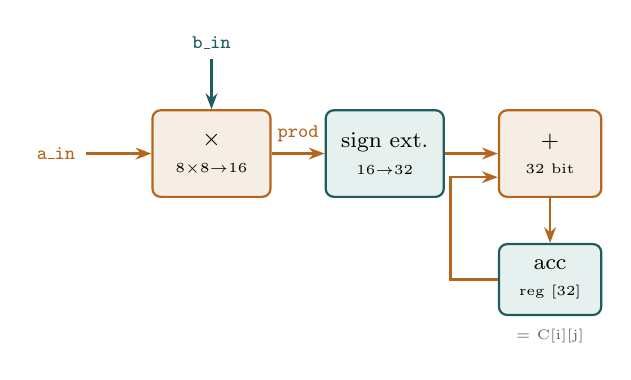
\begin{tikzpicture}[x=1mm,y=1mm]
      \node[hot, minimum width=15mm, minimum height=11mm] (mul) at (12,0)  {$\times$\\\tiny 8$\times$8$\to$16};
      \node[mod, minimum width=15mm, minimum height=11mm] (ext) at (34,0)  {sign ext.\\\tiny 16$\to$32};
      \node[hot, minimum width=13mm, minimum height=11mm] (add) at (55,0)  {$+$\\\tiny 32 bit};
      \node[mod, minimum width=13mm, minimum height=9mm]  (acc) at (55,-16) {acc\\\tiny reg [32]};
      \draw[wire]  (-4,0) node[left,font=\scriptsize\ttfamily]{a\_in} -- (mul.west);
      \draw[wireb] (12,12) node[above,font=\scriptsize\ttfamily]{b\_in} -- (mul.north);
      \draw[wire]  (mul) -- node[lbl,above=1mm]{prod} (ext);
      \draw[wire]  (ext) -- (add);
      \draw[wire]  (add) -- (acc);
      \draw[wire]  (acc.west) -- ++(-6,0) |- ([yshift=-3mm]add.west);
      \node[font=\tiny, text=muted, anchor=north] at (55,-21) {= C[i][j]};
    \end{tikzpicture}\\[3mm]
    \textbf{\footnotesize Pass-through path (to the neighbours)}\\[1mm]
    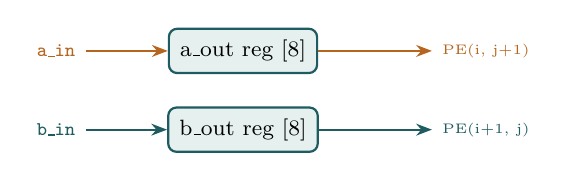
\begin{tikzpicture}[x=1mm,y=1mm]
      \node[mod, minimum width=15mm] (ar) at (20,0)  {a\_out reg [8]};
      \node[mod, minimum width=15mm] (br) at (20,-10) {b\_out reg [8]};
      \draw[wire]  (0,0)   node[left,font=\scriptsize\ttfamily]{a\_in} -- (ar);
      \draw[wireb] (0,-10) node[left,font=\scriptsize\ttfamily]{b\_in} -- (br);
      \draw[wire]  (ar) -- (44,0)   node[right,font=\tiny]{PE(i, j+1)};
      \draw[wireb] (br) -- (44,-10) node[right,font=\tiny]{PE(i+1, j)};
    \end{tikzpicture}
    \column{0.46\textwidth}\small
    \begin{itemize}
      \item \sig{prod = a\_in * b\_in}: both signed $\to$ a signed multiplier
            (one 9$\times$9 hard multiplier on MAX~10).
      \item Every enabled clock edge:\\
            \sig{acc <= acc + 32'(prod);}\\
            \sig{a\_out <= a\_in; b\_out <= b\_in;}
      \item \sig{clear} or reset $\to$ all three registers = 0.
      \item Worst case product: $(-128)\times(-128) = 16\,384$ fits in 16 bits;
            64 of them fit easily in 32 bits.
      \item Per PE: 32 + 8 + 8 = \textbf{48 flip-flops}.
    \end{itemize}
  \end{columns}
\end{frame}

% =====================================================================
\begin{frame}{Timing walk-through: when does each value reach each PE?}
  \small
  \begin{itemize}
    \item Read issued at step \textbf{t = k} $\to$ RAM data at \textbf{k + 1}
          $\to$ skew adds \textbf{i} (for A) or \textbf{j} (for B) $\to$ hops add \textbf{j} or \textbf{i}.
    \item So A[i][k] and B[k][j] \textbf{both} arrive at PE(i,j) at step
          \alert{\textbf{t = k + 1 + i + j}}: they always meet.
  \end{itemize}
  \vspace{1mm}
  \centering\scriptsize
  \begin{tabular}{@{}c c c c c@{}}
    \toprule
    \textbf{step t} & \textbf{state} & \textbf{RAM read} & \textbf{PE(0,0) gets} & \textbf{PE(3,3) gets} \\
    \midrule
    --- & CLEAR & --- & cleared to 0 & cleared to 0 \\
    0 & COMPUTE & k = 0 & 0 (zeros fed) & 0 \\
    1 & COMPUTE & k = 1 & A[0][0]$\cdot$B[0][0] & 0 \\
    7 & COMPUTE & k = 7 & A[0][6]$\cdot$B[6][0] & A[3][0]$\cdot$B[0][3] \\
    64 & DRAIN & --- & A[0][63]$\cdot$B[63][0] (last) & A[3][57]$\cdot$B[57][3] \\
    70 = K+2N$-$2 & DRAIN & --- & 0 & A[3][63]$\cdot$B[63][3] (last) \\
    --- & DONE & --- & C[0][0] final & C[3][3] final \\
    \bottomrule
  \end{tabular}\\[2mm]
  \raggedright\footnotesize
  N = 4, K = 64: CLEAR (1) + COMPUTE (64) + DRAIN (7) = \textbf{72 cycles = PERF\_TOTAL} $=$ 1.44\,\textmu s at 50\,MHz.
\end{frame}

% =====================================================================
\begin{frame}{Step 10 --- reading C back}
  \centering
  \resizebox{0.95\textwidth}{!}{%
  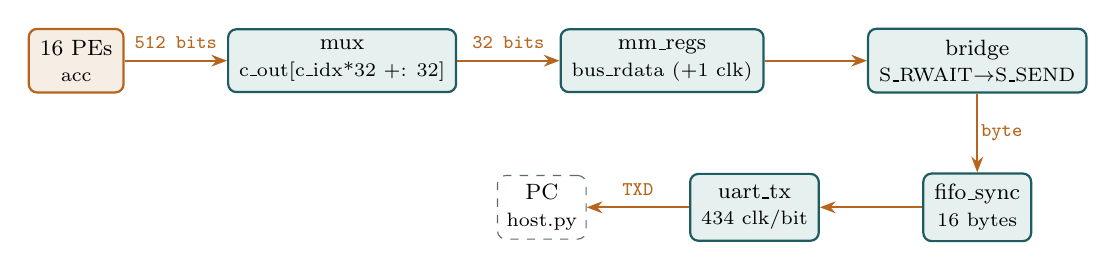
\begin{tikzpicture}[node distance=10mm and 13mm]
    \node[hot] (pe) {16 PEs\\\scriptsize acc};
    \node[mod, right=of pe] (mux) {mux\\\scriptsize c\_out[c\_idx*32 +: 32]};
    \node[mod, right=of mux] (rd) {mm\_regs\\\scriptsize bus\_rdata (+1 clk)};
    \node[mod, right=of rd] (br) {bridge\\\scriptsize S\_RWAIT$\to$S\_SEND};
    \node[mod, below=10mm of br] (q) {fifo\_sync\\\scriptsize 16 bytes};
    \node[mod, left=of q] (tx) {uart\_tx\\\scriptsize 434 clk/bit};
    \node[ext, left=of tx] (pc) {PC\\\scriptsize host.py};
    \draw[wire] (pe) -- node[lbl,above=1mm]{512 bits} (mux);
    \draw[wire] (mux) -- node[lbl,above=1mm]{32 bits} (rd);
    \draw[wire] (rd) -- (br);
    \draw[wire] (br) -- node[lbl,right]{byte} (q);
    \draw[wire] (q) -- (tx);
    \draw[wire] (tx) -- node[lbl,above=1mm]{TXD} (pc);
  \end{tikzpicture}}
  \vspace{3mm}
  \raggedright\small
  \begin{itemize}
    \item The host asks for address \sig{0x3000 + 4(i$\cdot$N + j)} $\to$ \sig{c\_idx = i$\cdot$N + j}
          selects one 32-bit accumulator.
    \item The bridge sends the 4 bytes little-endian through the 16-byte TX FIFO to \sig{uart\_tx}.
    \item 16 results $\times$ 4 bytes = 64 bytes $\approx$ 5.6\,ms over UART, compared with
          1.44\,\textmu s of compute $\to$ the design is \textbf{I/O-bound}.
  \end{itemize}
\end{frame}

% =====================================================================
\begin{frame}{Board I/O: \file{top\_de10lite.sv}}
  \begin{columns}[T]
    \column{0.5\textwidth}\small
    \begin{tabular}{@{}l l@{}}
      \toprule
      \textbf{Pin} & \textbf{Meaning} \\
      \midrule
      KEY0 & hold = reset (through sync\_2ff) \\
      HEX5..HEX0 & PERF\_COMPUTE of last job (hex) \\
      LEDR[2:0] & controller state (0..4) \\
      LEDR3 & busy \\
      LEDR5 & UART framing error (sticky) \\
      LEDR6 & unknown command (sticky) \\
      LEDR7 & host stalled mid-command \\
      LEDR8 & a job finished since reset \\
      LEDR9 & heartbeat, 1\,Hz (\sig{tick\_gen}) \\
      GPIO[0] / [1] & UART\_TXD / UART\_RXD \\
      \bottomrule
    \end{tabular}
    \column{0.47\textwidth}\small
    \begin{itemize}
      \item \sig{top\_de10lite} has \textbf{no logic of its own} beyond wiring and a few
            sticky flags: it connects pins $\to$ UART $\to$ bridge $\to$ core.
      \item Its port names (\sig{MAX10\_CLK1\_50}, \sig{KEY}, \sig{LEDR}, \sig{HEX0}...) must match
            the pin file \file{quartus/top\_de10lite.qsf}.
      \item Quartus builds it with \sig{N = 4, K\_MAX = 64} (set in \file{tools/gen\_quartus.py}).
      \item Expected after one job with K = 64: HEX shows \textbf{000047} (= 71).
    \end{itemize}
  \end{columns}
\end{frame}

% =====================================================================
\begin{frame}{One complete job, as the host sees it}
  \small
  \begin{enumerate}
    \item \sig{W 0x0008 K} \hfill set CFG\_K
    \item \sig{B 0x1000+i$\cdot$64 len=K bytes...}, once per row i \hfill load A (N block writes)
    \item \sig{B 0x2000 len=K$\cdot$N bytes...} \hfill load B
    \item \sig{W 0x0000 1} \hfill CTRL.START $\to$ controller leaves IDLE
    \item \sig{R 0x0004} until bit1 = 1 \hfill poll STATUS.DONE
    \item \sig{D 0x3000 len=4$\cdot$N$^2$} \hfill read C
    \item \sig{R 0x0010 ... 0x0020} \hfill read the 5 performance counters
  \end{enumerate}
  \vspace{2mm}
  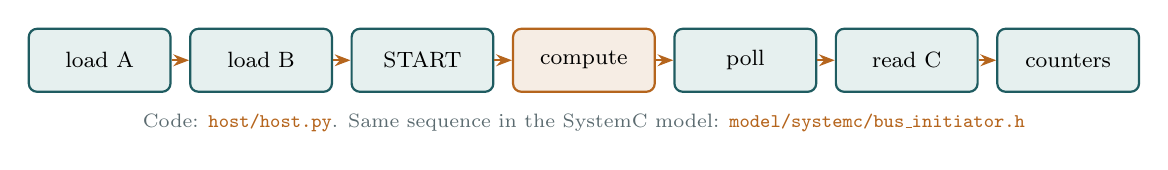
\begin{tikzpicture}
    \foreach \x/\t/\s in {0/load A/mod,1/load B/mod,2/START/mod,3/compute/hot,4/poll/mod,5/read C/mod,6/counters/mod} {
      \node[\s, minimum width=18mm, minimum height=8mm] (n\x) at (\x*2.05,0) {\t};
    }
    \foreach \a/\b in {0/1,1/2,2/3,3/4,4/5,5/6} \draw[wire] (n\a) -- (n\b);
    \node[font=\scriptsize, text=muted] at (6.15,-0.8) {Code: \file{host/host.py}. Same sequence in the SystemC model: \file{model/systemc/bus\_initiator.h}};
  \end{tikzpicture}
\end{frame}

% =====================================================================
\begin{frame}{RTL patterns used in this project (cheat sheet)}
  \begin{columns}[T]
    \column{0.5\textwidth}\scriptsize
    \resizebox{\linewidth}{!}{%
    \begin{tabular}{@{}l l@{}}
      \toprule
      \textbf{Pattern} & \textbf{Example file} \\
      \midrule
      Register (\sig{always\_ff}, \sig{<=}) & pe.sv accumulator \\
      Wires / mux (\sig{assign}, \sig{?:}) & mm\_core addr mux \\
      Combinational case (\sig{always\_comb}) & mm\_regs read mux \\
      FSM with \sig{typedef enum} & mm\_controller, uart\_rx, bridge \\
      Replication (\sig{for genvar}) & systolic\_array grid, RAM banks \\
      Parameters + \sig{\$clog2} & every core file \\
      Part-select \sig{[n*W +: W]} & flat lane buses \\
      Valid/ready handshake & register bus, uart\_tx \\
      2-FF synchronizer & sync\_2ff (KEY, UART\_RXD) \\
      Inferred block RAM & sram\_sp \\
      \bottomrule
    \end{tabular}}
    \column{0.47\textwidth}\small
    \textbf{Rules the code follows}
    \begin{itemize}
      \item One clock (50\,MHz), synchronous active-low reset.
      \item \sig{<=} only in \sig{always\_ff}; \sig{=} only in \sig{always\_comb}.
      \item Every \sig{case} has a \sig{default} $\to$ no latches.
      \item External inputs are synchronized before use.
      \item Pulses (\sig{start}, \sig{done}, \sig{valid}) last exactly one cycle.
      \item No clock is made from logic: slow events use a \textbf{tick enable}.
    \end{itemize}
  \end{columns}
\end{frame}

% =====================================================================
\begin{frame}{Your learning path through the RTL}
  \scriptsize
  \begin{tabular}{@{}c p{30mm} p{50mm} p{48mm}@{}}
    \toprule
    \textbf{\#} & \textbf{Read} & \textbf{Look for} & \textbf{Try (on Ubuntu)} \\
    \midrule
    1 & pe.sv & multiply, accumulate, pass-through regs & \sig{pytest tb/test\_pe.py}, open waves \\
    2 & systolic\_array.sv & how genvar loops wire 16 PEs & draw the 4$\times$4 grid yourself \\
    3 & skew\_buffer.sv & lane n delayed n cycles & \sig{pytest tb/test\_skew\_buffer.py} \\
    4 & sram\_sp.sv & 1-cycle read latency & explain why \sig{rd\_valid} exists \\
    5 & mm\_controller.sv & 5 states, counter t, all\_active & derive K + 2N on paper \\
    6 & mm\_regs.sv & address split, counters & decode 0x2017 by hand (= B[5][3]) \\
    7 & mm\_core.sv & how 1--6 connect & trace one value from RAM to PE(3,3) \\
    8 & uart\_rx/tx.sv & 434 clocks per bit & \sig{pytest tb/test\_uart\_rx.py} \\
    9 & uart\_bus\_bridge.sv & command FSM & send a \texttt{P} command in the test \\
    10 & top\_de10lite.sv & board wiring, LEDs, HEX & \sig{tools/build.sh}, program board \\
    \bottomrule
  \end{tabular}
  \vspace{2mm}

  \small\textbf{Exercise:} change \sig{2N-1} to \sig{2N-2} in \file{mm\_controller.sv}, run the tests,
  see which one fails, then undo it. (Answer: the FILLDRAIN counter check.)
\end{frame}

% =====================================================================
\begin{frame}{Key numbers to remember}
  \centering
  \tikzset{stat/.style={hot, minimum width=32mm, minimum height=20mm, align=center}}
  \begin{tikzpicture}
    \node[stat] at (0,0)    {\Large\bfseries 16 PEs\\[1mm]\scriptsize\color{muted} N = 4 build (64 at N = 8)};
    \node[stat] at (3.6,0)  {\Large\bfseries 72 cycles\\[1mm]\scriptsize\color{muted} one job: N = 4, K = 64};
    \node[stat] at (7.2,0)  {\Large\bfseries 90.1\,\%\\[1mm]\scriptsize\color{muted} PE utilisation (N = 4)};
    \node[stat] at (10.8,0) {\Large\bfseries 434\\[1mm]\scriptsize\color{muted} clocks per UART bit};
  \end{tikzpicture}
  \vspace{5mm}
  \raggedright\small
  \begin{itemize}
    \item \textbf{Data path:} UART $\to$ bridge $\to$ bus $\to$ mm\_regs $\to$ RAM banks $\to$ skew
          $\to$ 16 PEs $\to$ mux $\to$ bus $\to$ bridge $\to$ UART.
    \item \textbf{Control path:} mm\_regs (START) $\to$ mm\_controller $\to$ clear / rd\_en / array\_en
          $\to$ counters.
    \item \textbf{One formula:} a value from read step k meets in PE(i,j) at step k + 1 + i + j.
  \end{itemize}
\end{frame}

\end{document}
